
%%% Local Variables:
%%% mode: latex
%%% TeX-master: t
%%% End:


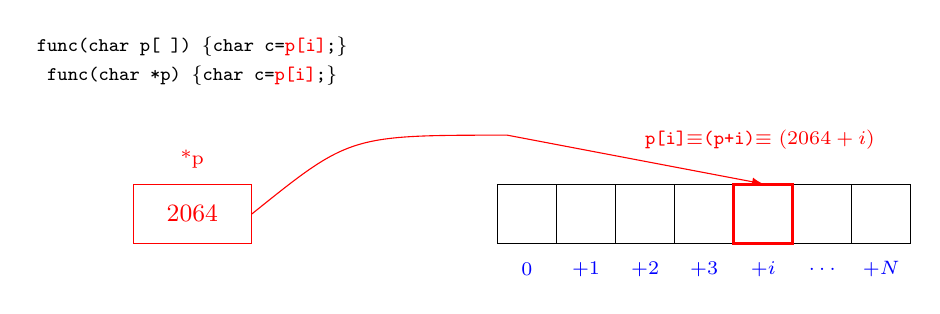
\begin{tikzpicture}

\def\offset{.75cm}
\def\addr{2064}

\tikzset{
        every node/.style={font=\scriptsize},
        every path/.style={->,>=latex,draw},
        data/.style={minimum height=.75cm, draw},
        pointer/.style={data,font=\small,red,minimum width=2*\offset},
        array/.style={data,minimum width=\offset},
        index/.style={blue}
}

\node[pointer] (P) at (0,0) {2064};
\node[red] (pointer label) [above of=P,yshift=-\offset/2.5] {*p};

\node (MEM) [right of=P,xshift=3*\offset] {};

\foreach \i/\l in {0/0,1/+1,2/+2,3/+3,4/+$i$,5/$\ldots$,6/+$N$} {
     \node[array] (A\i) [right of=MEM,xshift=\i*\offset] {};
     \node[index] [below of=A\i,yshift=\offset/2.5] {\l};
}

\draw[red] (P.east) .. controls (2,1) .. (4,1)  --  node[above
right,red] {\tt p[i]$\equiv$(p+i)$\equiv(2064+i)$}  (A4.north);

\node[array,red, very thick] at (A4) {};

\node [above of=P,yshift=1.5*\offset] {\tt func(char p[ ]) \{char c={\color{red}p[i]};\}};
\node [above of=P,yshift=\offset] {\tt func(char *p) \{char c={\color{red}p[i]};\}};

\end{tikzpicture}
